\section{洛朗级数}

\begin{theorem}[Laurant 定理]
在圆环 $H:r<\lvert z-a \rvert<R(r\geq0,R\leq+\infty)$ 内解析的函数 $f(z)$ 必可以展开成双边幂级数,即\textbf{Laurant 级数}
\[
f(z)=\sum_{n=-\infty}^{\infty} c_n(z-a)^{n}
\]
其中\textbf{Laurant 系数}
\[
c_n=\frac{1}{2\pi i} \oint_{C} \frac{f(\zeta)}{(\zeta-a)^{n+1}} \, \mathrm{d}\zeta \qquad (n=0,\pm1,\pm2,\dots) 
\]
$C$ 为圆周 $\lvert \zeta-a \rvert=\rho(r<\rho<R)$,并且展开式唯一.
\end{theorem}
展开洛朗级数直接暴力展开即可.

\subsection{奇点}

\begin{figure}[H]
\centering
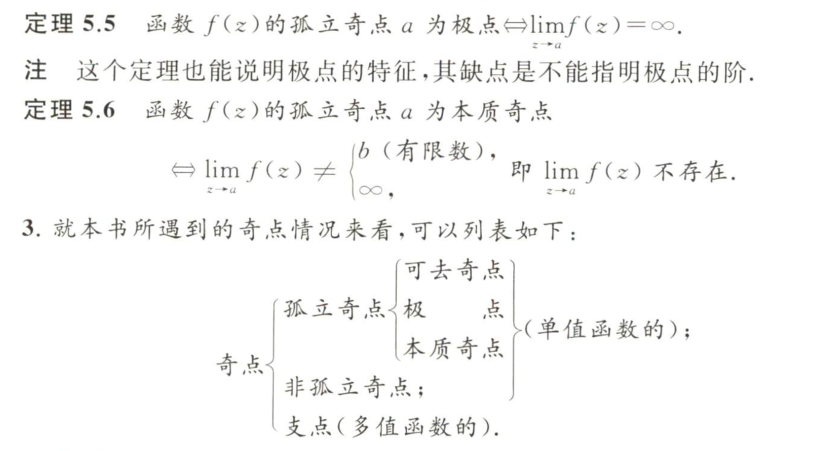
\includegraphics[width=\textwidth]{1-洛朗级数-2025040612.png}
% \caption{}
\label{}
\end{figure}
\begin{figure}[H]
\centering
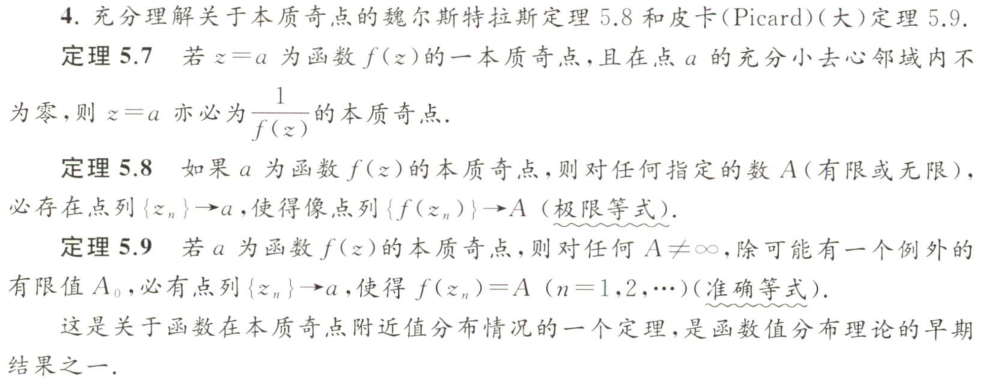
\includegraphics[width=\textwidth]{洛朗级数-2025040612.png}
% \caption{}
\label{}
\end{figure}

\subsubsection{判断奇点特性}

\begin{figure}[H]
\centering
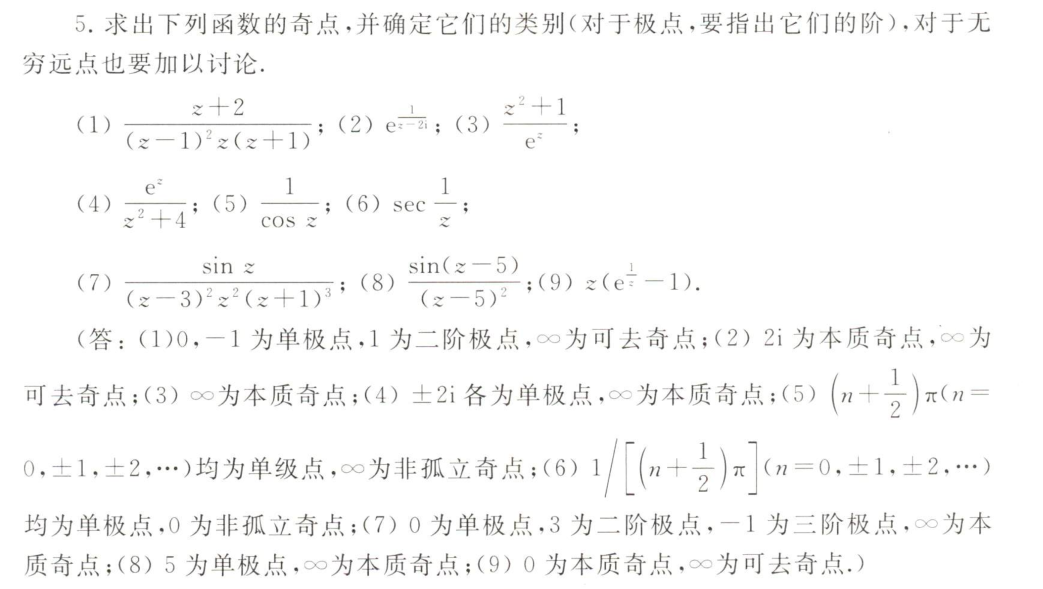
\includegraphics[width=\textwidth]{6-洛朗级数-2025040616.png}
% \caption{}
\label{}
\end{figure}
\begin{figure}[H]
\centering
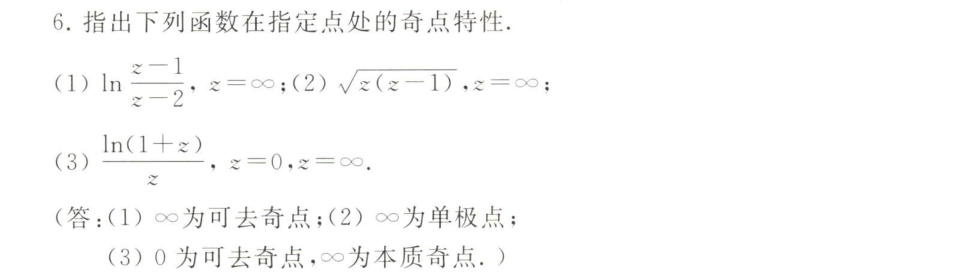
\includegraphics[width=\textwidth]{5-洛朗级数-2025040616.png}
% \caption{}
\label{}
\end{figure}

\subsection{解析函数在无穷远点处的性质}

由于函数 $f(z)$ 在 $\infty$ 总是无意义的,所以点 $\infty$ 总是 $f(z)$ 的奇点.

\subsubsection{Example 1}

对于函数
\[
f(z)=\frac{z^{6}+1}{z(z^2+1)^2}
\]
它是有理分式函数,分母的零点 $0,i,-i$ 是这个函数的极点,下面考虑它们的阶.

$z=0$ 是分母的一阶零点,且不是分子 $z^6+1$ 的零点,故 $z=0$ 是 $f(z)$ 的一阶极点. 注意到 $z^{6}+1=(z^2+1)(z^{4}-z^2+1)$,
\[
\frac{z^{6}+1}{z(z^2+1)^2}=\frac{z^{4}-z^2+1}{z(z-i)[z-(-i)]}
\]
于是 $z=i,z=-i$ 也是 $f(z)$ 的一阶极点.

接下来考虑 $\infty$,因为
\[
\frac{z^{6}+1}{z(z^2+1)^2}=\frac{z^{6}\left( 1+\frac{1}{z^{6}}  \right)}{z^{5}\left( 1+\frac{2}{z^2}+\frac{1}{z^{4}}  \right)}=z\left( 1-\frac{2}{z^{2}}+\dots \right)
\]
其中 $\mu(z)=1-\frac{2}{z^2}+\dots$ 在 $z=\infty$ 解析,且 $\mu(\infty)=1\neq0$,因此 $z=\infty$ 是 $f(z)$ 的一阶零点.

\subsubsection{Example 2}

对于函数
\[
f(z)=\frac{1}{z^2}+\frac{1}{z^3}
\]
它只有 $z=0,z=\infty$ 作为奇点,$z=0$ 作为 $f(z)$ 的三阶极点,$f(z)$ 在 $z=\infty$ 的主要部分 (即正幂) 为\textbf{零},故 $z=\infty$ 是 $f(z)$ 的可去奇点.

由于 $\frac{1}{f(z)}=z^2\left( 1-\frac{1}{z+1} \right)$ 以 $z=\infty$ 为二阶极点,故 $f(z)$ 以 $z=\infty$ 为二阶零点.

\subsubsection{Example 3}

对于函数
\[
f(z)=\frac{1}{1+e^{ z }}
\]
解 $1+e^{ z }=0$ 得到 $\frac{1}{f(z)}$ 的零点
\[
z_k=(2k+1)\pi i \qquad (k=0,\pm1,\pm2,\dots)
\]
又因为 $\left.(1+e^{ z })'\right|_{z=z_k}\neq0$,所以 $z_k$ 都是 $\frac{1}{f(z)}$ 的一阶零点. 于是 $z_k$ 都是 $f(z)$ 的一阶极点.

当 $k\to \infty$ 时,$z_k\to \infty$. 故点 $\infty$ 是 $f(z)$ 的非孤立奇点,即极点列 $\{ z_k \}$ 的聚点.

\subsubsection{多值函数的洛朗展式}

\begin{figure}[H]
\centering
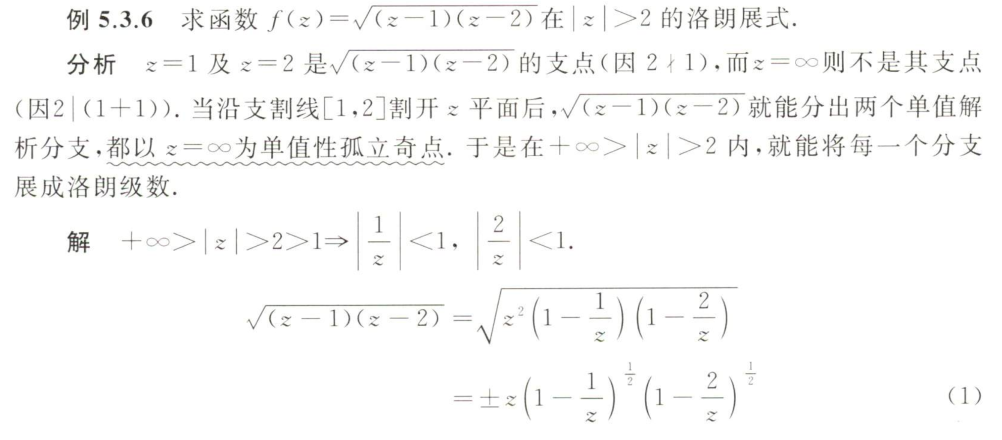
\includegraphics[width=\textwidth]{洛朗级数-2025040614.png}
% \caption{}
\label{}
\end{figure}

\begin{figure}[H]
\centering
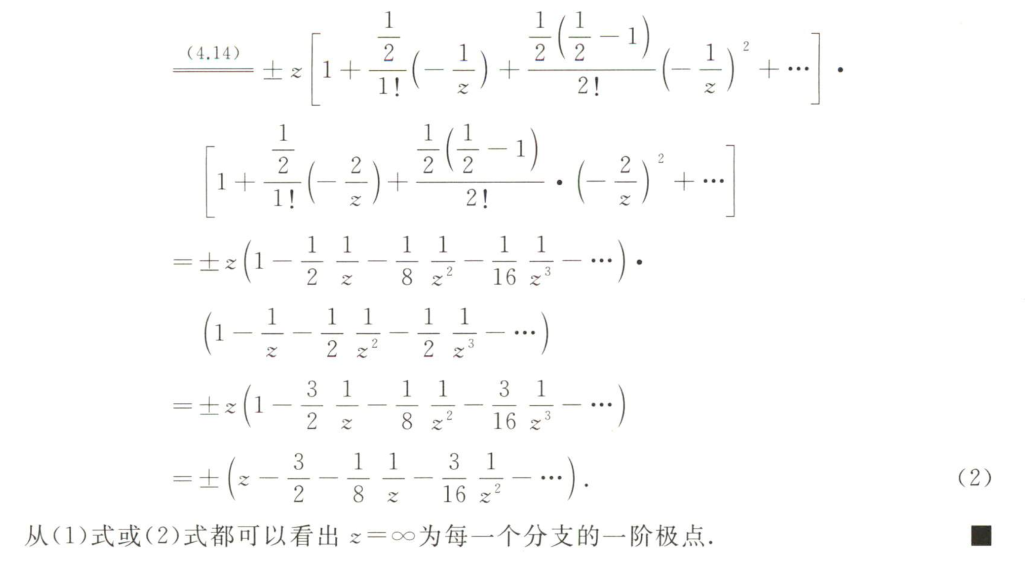
\includegraphics[width=\textwidth]{1-洛朗级数-2025040614.png}
% \caption{}
\label{}
\end{figure}

\subsubsection{通过洛朗展式判断极点阶数}

\begin{figure}[H]
\centering
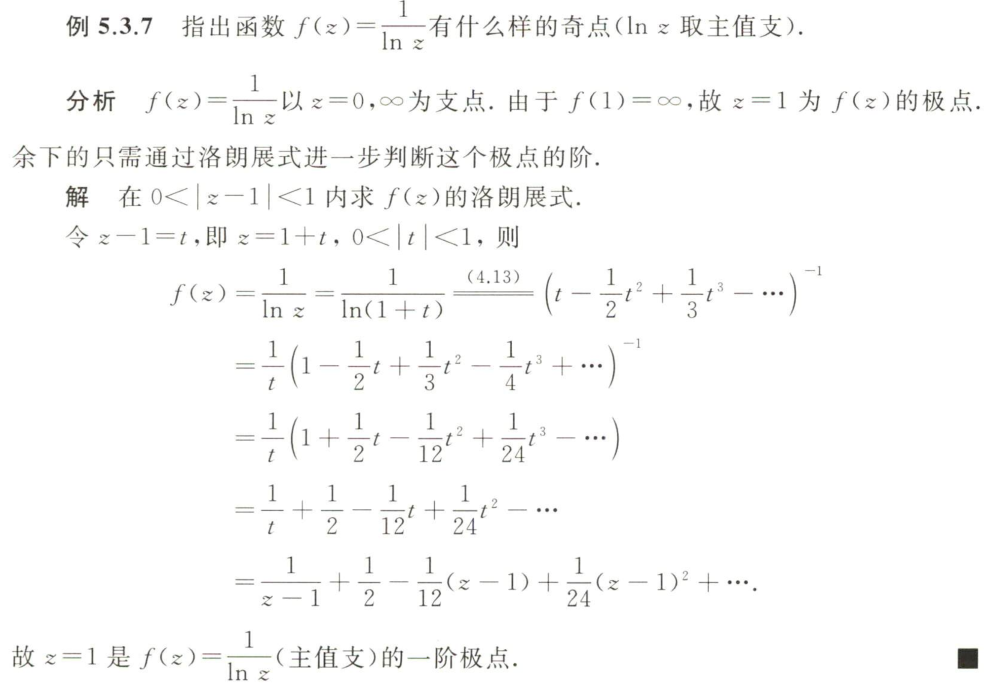
\includegraphics[width=\textwidth]{2-洛朗级数-2025040614.png}
% \caption{}
\label{}
\end{figure}

\subsection{整函数与亚纯函数}

\begin{figure}[H]
\centering
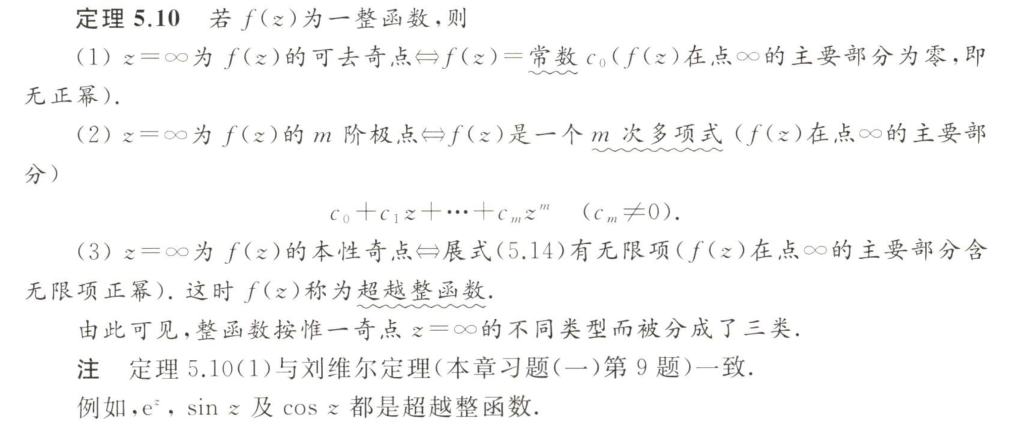
\includegraphics[width=\textwidth]{4-洛朗级数-2025040616.png}
% \caption{}
\label{}
\end{figure}

\subsubsection{整函数可表示为 \texorpdfstring{$f(z)=A+e^{ g(z) }$}{f(z)=A+e^ g(z)}}

\begin{figure}[H]
\centering
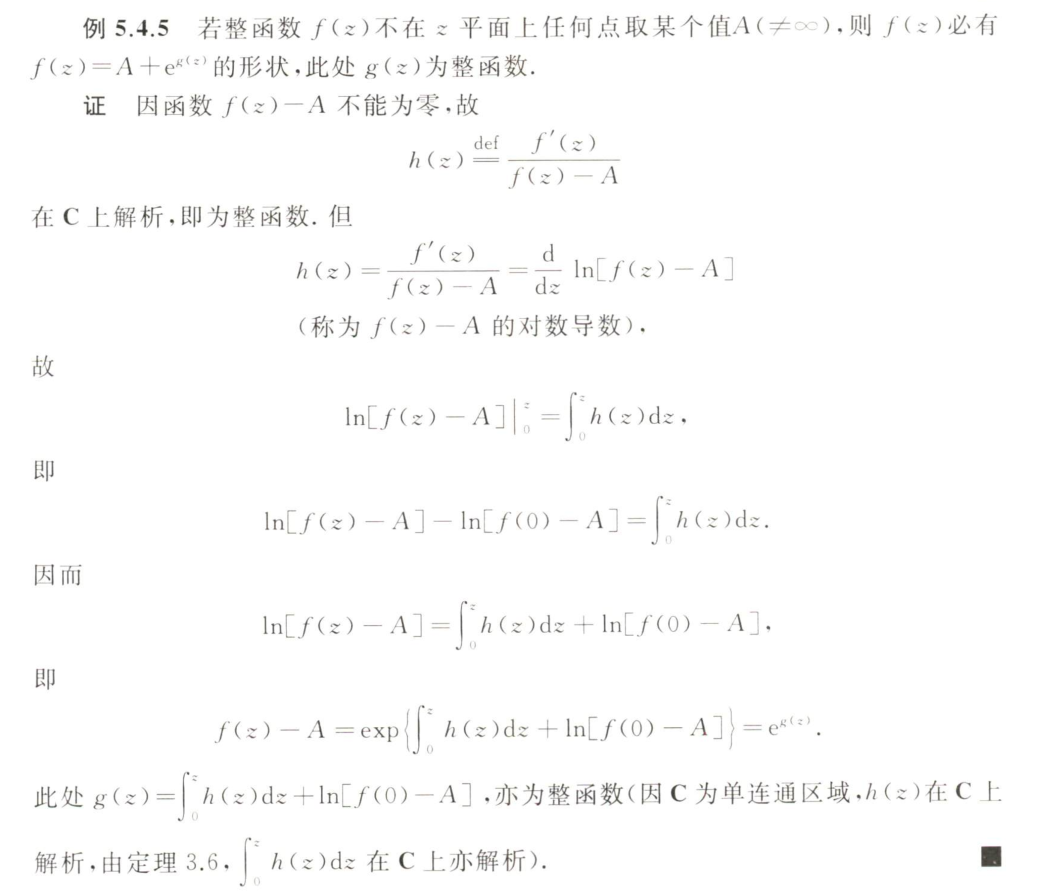
\includegraphics[width=\textwidth]{3-洛朗级数-2025040614.png}
% \caption{}
\label{}
\end{figure}

\subsubsection{证明 \texorpdfstring{$O(1)$}{O(1)} 的整函数有零点}

\begin{exercise}
设 $f\in H(\mathbb{C})$,当 $z\to \infty$ 时 $\frac{f(z)}{z}\to1$. 证明:$f(z)$ 必有一个零点.
\end{exercise}
\begin{proof}
由于 $f$ 是整函数,故只有 $z=\infty$ 作为孤立奇点,于是可设
\[
f(z)=c_0+c_1+c_2z^2+\dots+c_nz^{n}+\dots \qquad 0\leq \lvert z \rvert <\infty
\]
又由题设
\[
\lim_{ z \to \infty } \frac{f(z)}{z}=1
\]
可见 $z=\infty$ 为 $\frac{f(z)}{z}$ 的可去奇点,从而 $z=\infty$ 为 $f(z)$ 的一阶极点,从而
\[
f(z)=c_0+z
\]
于是 $f(z)$ 必然有且仅有一个零点.

\end{proof}

\subsubsection{亚纯函数在周线 \texorpdfstring{$C$}{C} 内只有有限个零点和极点}

\begin{figure}[H]
\centering

\includegraphics[width=\textwidth]{4-洛朗级数-2025040614.png}
% \caption{}
\label{}
\end{figure}
\begin{figure}[H]
\centering
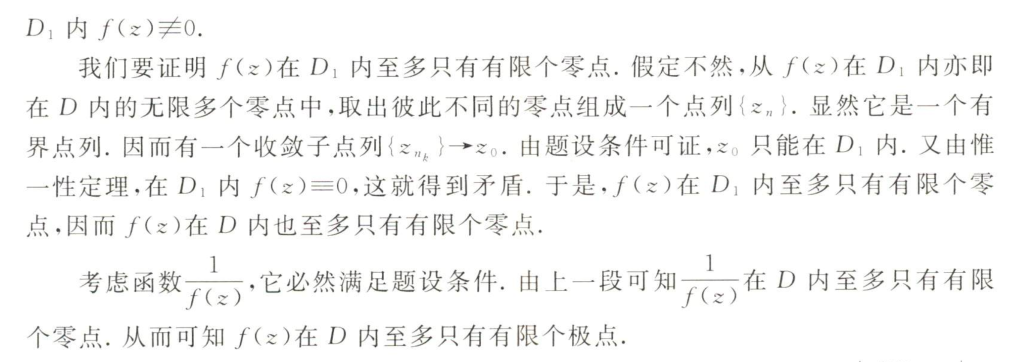
\includegraphics[width=\textwidth]{5-洛朗级数-2025040614.png}
% \caption{}
\label{}
\end{figure}

\subsection{Schwarz lemma}

\href{https://fr.wikipedia.org/wiki/Lemme_de_Schwarz#Preuve}{Lemme de Schwarz — Wikipédia}

\subsubsection{Statement}

Let $f: \mathbb{D} \rightarrow \mathbb{C}$ be a holomorphic function on the open unit disk
\[
\mathbb{D}=\{z \in \mathbb{C}:|z|<1\}
\]
Such that:

\begin{enumerate}
	\item $f(0)=0$,
	\item $|f(z)| \leq 1$ for all $z \in \mathbb{D}$.
\end{enumerate}

Then:

\begin{enumerate}
	\item $|f(z)| \leq|z|$ for all $z \in \mathbb{D}$,
	\item $\left|f^{\prime}(0)\right| \leq 1$,
	\item Moreover, if equality holds at any point other than 0 (i.e., if $|f(z)|=|z|$ for some $z \neq 0$ ), or if $\left|f^{\prime}(0)\right|=1$, then $f(z)=e^{i \theta} z$ for some real constant $\theta$.
\end{enumerate}

\begin{note}
If $\lvert f(z) \rvert=1$ for some $\lvert z \rvert=1$, $f$ may not be a rotation. Consider $f(z)=z^{n}$; it satisfies the conditions, and $\lvert f(e^{ i\alpha }) \rvert=\lvert e^{ in\alpha } \rvert=1=\lvert e^{ i\alpha } \rvert$, but $f(z)\neq e^{ i\theta }z$.
\end{note}
\subsubsection{Proof}

The proof is \underline{a straightforward application of the maximum modulus principle} on the function
\[
g(z)= \begin{cases}\frac{f(z)}{z} & \text { if } z \neq 0 \\ f^{\prime}(0) & \text { if } z=0\end{cases}
\]
which is holomorphic on the whole of $D$, including at the origin (because $f$ is differentiable at the origin and fixes zero). Now if $D_r=\{z:|z| \leq r\}$ denotes the closed disk of radius $r$ centered at the origin, then the maximum modulus principle implies that, for $r<1$, given any $z \in D_r$, there exists $z_r$ on the boundary of $D_r$ such that
\[
|g(z)| \leq\left|g\left(z_r\right)\right|=\frac{\left|f\left(z_r\right)\right|}{\left|z_r\right|} \leq \frac{1}{r}
\]
As $r \rightarrow 1$ we get $|g(z)| \leq 1$.

Moreover, suppose that $|f(z)|=|z|$ for some non-zero $z \in D$, or $\left|f^{\prime}(0)\right|=1$. Then, $|g(z)|=1$ at some point of $D$. So by the maximum modulus principle, $g(z)$ is equal to a constant $a$ such that $|a|=1$. Therefore, $f(z)=a z$, as desired.

\subsubsection{General Schwarz lemma}

If $f\in H(B_{R}(z_0)),f(z_0)=0,\lvert f(B_{R}(z_0)) \rvert\leq M$, then let
\[
g:\mathbb{D}\to \mathbb{D}\qquad z\mapsto\frac{1}{M}f\left(Rz+z_0 \right)
\]
Then $g(0)=0,\lvert g(\mathbb{D}) \rvert\leq1$. Apply Schwarz lemma,
\[
\lvert \underbrace{ g(z) }_{ =M^{-1}f(Rz+z_0) } \rvert \leq \lvert z \rvert \qquad \lvert \underbrace{ g'(0) }_{ =RM^{-1}f'(z_0) } \rvert \leq 1
\]
i.e.
\[
\lvert f(z) \rvert \leq \frac{M}{R}\lvert z-z_0 \rvert ,\forall z\in B(z_0,R)\qquad \lvert f'(z_0) \rvert \leq 1
\]
\subsection{Schwarz 引理的应用}

\begin{exercise}[cmc 第八届高年级决赛]
设函数 $f(z)$ 在单位圆 $\lvert z \rvert<1$ 内解析,并且 $\lvert f(z) \rvert\leq M(M>0)$,$M$ 为常数. 证明:
\[
\lvert f'(0) \rvert \leq M-\frac{\lvert f(0) \rvert ^2}{M}
\]
\end{exercise}
\begin{proof}
令 $w=w(z)=\frac{f(z)}{M}$,做变换
\[
F(z)=\frac{w(z)-w(0)}{1-\overline{w(0)}w(z)}\qquad \text{where }w(0)=\frac{f(0)}{M}
\]
则该变换将单位圆 $\lvert w \rvert<1$ 映射为 $\lvert F(z) \rvert<1$. 由 Schwarz 引理 $\lvert F'(0) \rvert\leq1$. 由于
\[
\begin{aligned}
\left.F'(z)\right|_{z=0} & =\left.\left( \frac{w(z)-w(0)}{1-\overline{w(0)}w(z)} \right)'\right|_{z=0}=\lim_{ z \to 0 } \left( \frac{\frac{w(z)-w(0)}{z}}{1-\overline{w(0)}w(z)} \right)=\frac{w'(0)}{1-\lvert w(0) \rvert ^2} \\
 & =\frac{f'(0)M}{M^2-\lvert f(0) \rvert ^2} 
\end{aligned}
\]
则
\[
\left\lvert  \frac{f'(0)M}{M^2-\lvert f(0) \rvert ^2}  \right\rvert \leq 1\implies \lvert f'(0) \rvert M\leq \lvert M^2-\lvert f(0) \rvert ^2 \rvert=M^2-\lvert f(0) \rvert ^2
\]
从而
\[
\lvert f'(0) \rvert \leq M-\frac{\lvert f(0) \rvert ^2}{M}
\]
\end{proof}

\subsubsection{推广到 \texorpdfstring{$k$}{k} 阶导数}

\begin{figure}[H]
\centering
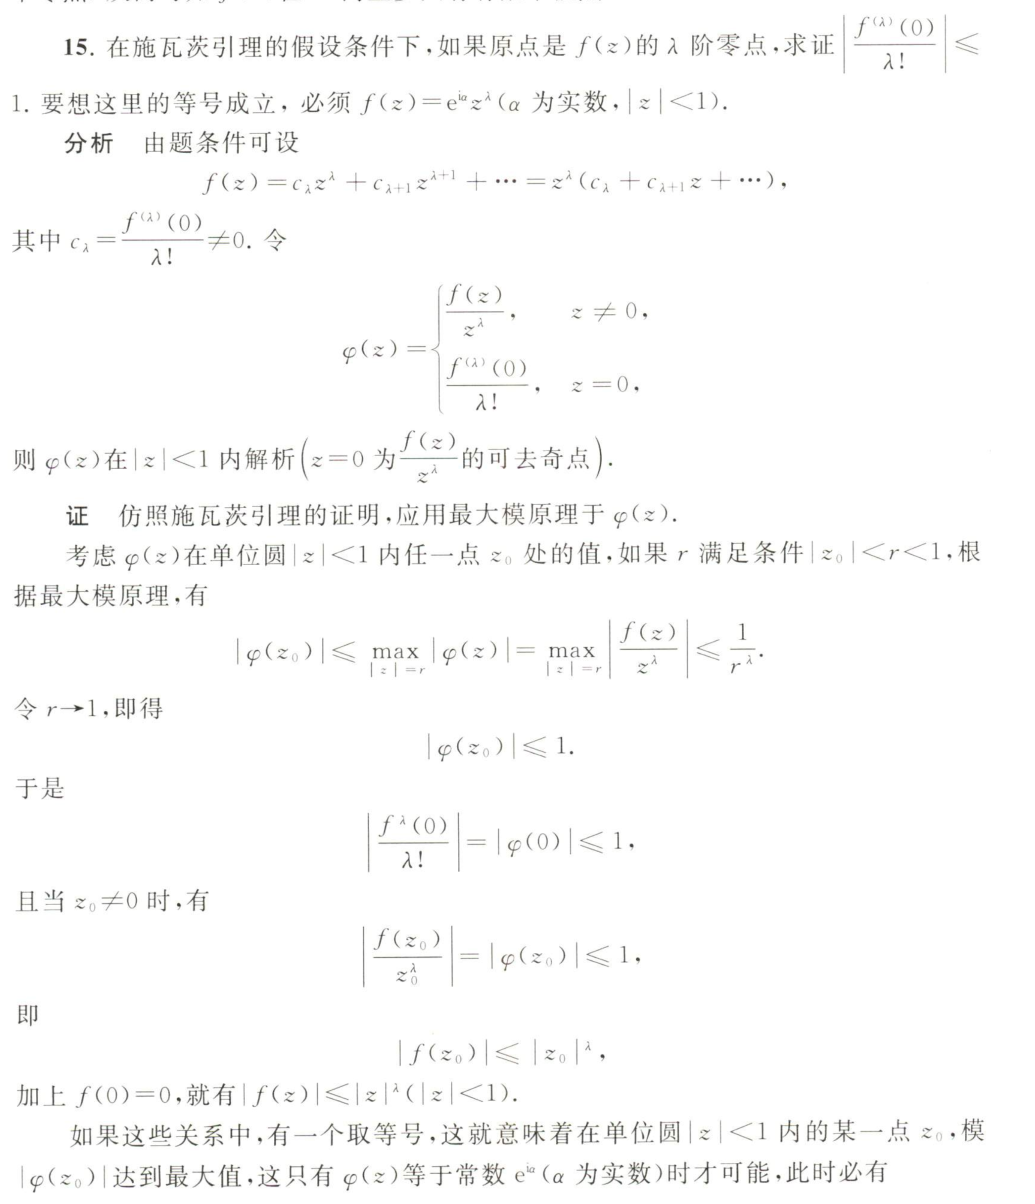
\includegraphics[width=\textwidth]{洛朗级数-2025040616.png}
% \caption{}
\label{}
\end{figure}

\begin{figure}[H]
\centering

\includegraphics[width=\textwidth]{2-洛朗级数-2025040616.png}
% \caption{}
\label{}
\end{figure}

\subsubsection{课堂练习}

\begin{exercise}
设 $f(z)$ 在 $\lvert z \rvert<1$ 内解析,$f(0)=0$,$\lvert \mathrm{Re}f(z) \rvert<1$, 则 $\lvert f'(0) \rvert\leq\frac{4}{\pi}$.
\end{exercise}
这类涉及解析函数在特定区域(通常是单位圆盘)内满足某些条件(如 $f(0)=0$ 和其值域受限),并要求证明其导数在某点(通常是原点)的模有界的题目,通常采用以下标准解题方法:

\paragraph{解题步骤 📝}

\begin{enumerate}
	\item \textbf{确定函数的定义域和值域限制}
	\begin{itemize}
		\item \textbf{定义域 (D)}:通常是单位圆盘 $|z| < 1$。
		\item \textbf{标准化条件}:常见的有 $f(0) = 0$。
		\item \textbf{值域 (S)}:根据题目条件确定 $f(z)$ 的取值范围。例如,$|Re(f(z))| < A$ 表示值域是带形区域 $\{-A < Re(w) < A\}$;$|f(z)| < M$ 表示值域是圆盘 $|w| < M$;$Re(f(z)) > 0$ 表示值域是右半平面。
	\end{itemize}
	\item \textbf{构造辅助保形映射 (Conformal Mapping)} 🗺️
	\begin{itemize}
		\item 寻找一个解析函数 $H(w)$,它能将 $f(z)$ 的值域 $S$ \textbf{保形地映射}到单位圆盘 $D'$ ($|\zeta| < 1$)。
		\item 这个映射 $H(w)$ 需要将对应于 $f(0)$ 的点(在$S$中,通常是0点)映射到单位圆盘 $D'$ 的原点。即,如果 $f(0) = w_0$ (在$S$中),则需要 $H(w_0) = 0$。在常见的 $f(0)=0$ 条件下,我们需要 $H(0)=0$。
	\end{itemize}
	\item \textbf{构造复合函数} 🧩
	\begin{itemize}
		\item 定义一个新的函数 $G(z) = H(f(z))$。
		\item \textbf{验证 $G(z)$ 的性质}:
		\begin{itemize}
			\item $G(z)$ 在原定义域 $D$ ($|z| < 1$) 内解析(因为 $f$ 和 $H$ 均解析)。
			\item $G(0) = H(f(0)) = H(0) = 0$ (利用标准化条件和 $H$ 的选取)。
			\item $G(z)$ 将单位圆盘 $D$ 映射到单位圆盘 $D'$ ($|G(z)| < 1$ for $|z| < 1$)。
		\end{itemize}
	\end{itemize}
	\item \textbf{应用施瓦茨引理 (Schwarz's Lemma)} ✨
	\begin{itemize}
		\item 由于 $G(z)$ 满足施瓦茨引理的条件(解析于 $|z|<1$, $G(0)=0$, $|G(z)| \le 1$),我们可以得到结论:
		\begin{itemize}
			\item $|G(z)| \le |z|$ for all $z$ in $D$.
			\item \textbf{$|G'(0)| \le 1$} (这是最关键的一步,用于求解导数界限)。
		\end{itemize}
	\end{itemize}
	\item \textbf{计算导数并建立不等式} ⚙️
	\begin{itemize}
		\item 使用链式法则计算 $G'(z)$:$G'(z) = H'(f(z)) \cdot f'(z)$。
		\item 在 $z=0$ 处取值:$G'(0) = H'(f(0)) \cdot f'(0)$。由于 $f(0)=0$,则 $G'(0) = H'(0) \cdot f'(0)$。
		\item 将此代入施瓦茨引理的结论:$|H'(0) \cdot f'(0)| \le 1$。
		\item 从而得到:$|H'(0)| \cdot |f'(0)| \le 1$。
	\end{itemize}
	\item \textbf{求解目标界限} 🎯
	\begin{itemize}
		\item 从上一步的不等式解出 $|f'(0)|$:
$|f'(0)| \le 1 / |H'(0)|$。
		\item $|H'(0)|$ 是一个具体的数值,取决于所构造的保形映射 $H(w)$。计算出这个值,即可得到 $|f'(0)|$ 的上界。
	\end{itemize}
	\item \textbf{讨论等号成立条件 (Sharpness)} 🧐
	\begin{itemize}
		\item 等号 $|f'(0)| = 1 / |H'(0)|$ 成立当且仅当施瓦茨引理中的等号 $|G'(0)| = 1$ 成立。
		\item 这要求 $G(z) = \lambda z$,其中 $|\lambda|=1$ 是一个常数。
		\item 因此,$H(f(z)) = \lambda z$,即 $f(z) = H^{-1}(\lambda z)$。
		\item 这意味着使等号成立的函数 $f(z)$ 是将单位圆盘 $D$ 保形映射(可能经过一个旋转 $\lambda$)到区域 $S$ 的那些\textbf{极值函数}。
		\item 这个分析有助于判断题目要求的 $<$(严格小于)还是 $\le$(小于等于)是否准确,并理解不等式的精确性。
	\end{itemize}
\end{enumerate}


\paragraph{常用保形映射示例:}

\begin{itemize}
	\item \textbf{带形 $|Re(w)| < A$ 到单位圆盘 $|\zeta|<1$,且 $w=0$ 映到 $\zeta=0$}:
$H(w) = \tanh(i\pi w / (4A))$ 或 $H(w) = (e^{i\pi w/(2A)} - 1) / (e^{i\pi w/(2A)} + 1)$。
对于 $A=1$, $H(w) = \tanh(i\pi w/4)$,则 $|H'(0)| = \pi/4$。
	\item \textbf{右半平面 $Re(w) > 0$ 到单位圆盘 $|\zeta|<1$,且 $w=1$ 映到 $\zeta=0$} (需调整以使 $w=0$ (如果 $f(0)=0$ 且 $0$ 在边界) 或某特定点映射到0):
典型的如 $\zeta = (w-1)/(w+1)$ (这映射 $Re(w)>0$ 到 $|\zeta|<1$,且 $w=1$ 到 $\zeta=0$)。如果 $f(0)$ 的像点在$S$中的某个位置 $w_0$,需要调整映射使得 $H(w_0)=0$。
\end{itemize}


通过这套流程,大部分此类问题都可以得到系统性的解决。关键在于正确识别 $f(z)$ 的值域 $S$ 并找到合适的保形映射 $H(w)$。

\subsection{Schwarz lemma and automorphisms of the disk}

\href{https://www.ma.imperial.ac.uk/~dcheragh/Teaching/2016-F-GCA/2016-F-GCA-Ch2.pdf}{LectureNotes}

We have see that every rotation $z\mapsto e^{ i\theta }\cdot z$, for fixed $\theta\in \mathbb{R}$, is an automorphism of the disk. For $a\in \mathbb{D}$ define
\[
\varphi_{a}(z)=\frac{a-z}{1-\overline{a}z}
\]
which is also an automorphism of $\mathbb{D}$.

When $\lvert z \rvert=1$, we have
\[
\lvert \varphi_{a}(z) \rvert =\left\lvert  \frac{a-z}{1-\overline{a}z}  \right\rvert =\left\lvert  \frac{a-z}{\overline{z}-\overline{a}}  \right\rvert \cdot \lvert \overline{z} \rvert =1
\]
Observe that
\[
\varphi_{a}(a)=0\qquad \varphi_{a}(0)=a
\]
Then
\[
\varphi_{a}\circ \varphi_{a}(0)=0\qquad \varphi_{a}\circ \varphi_{a}(a)=a
\]
By the Schwarz lemma, $\varphi _a\circ\varphi_{a}:z\mapsto e^{ i\theta }z$, and $\theta=0$. Thus $\varphi_{a}\circ\varphi_{a}$ is identity map of $\mathbb{D}$. It follows that $\varphi_{a}$ is bijection from $\mathbb{D}$ to $\mathbb{D}$.

\begin{theorem}[Automorphism of $\mathbb{D}$]
A map $f$ is an automorphism of $\mathbb{D}$ iff there are $\theta\in \mathbb{R}$ and $a\in \mathbb{D}$ s.t.
\[
f(z)=e^{ i\theta }\cdot\frac{a-z}{1-\overline{a}z}
\]
\end{theorem}
\subsubsection{Properties of \texorpdfstring{$\varphi_{a}$}{varphi_a}}

\begin{remark}
这里的 $\varphi_{a}$ 和前面的定义差了一个负号,导致之前的 $\varphi_{a}$ 是幂等映射,而这里的 $\varphi_{a}$ 的逆为 $\varphi_{-a}$.
\end{remark}
\begin{figure}[H]
\centering
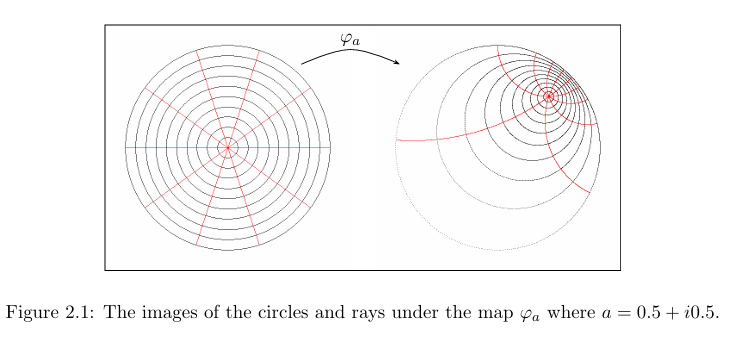
\includegraphics[width=\textwidth]{洛朗级数-2025041018.png}
% \caption{}
\label{}
\end{figure}
\[
\varphi_{a}(z)=\frac{z-a}{1-\overline{a}z}
\]
\[
\varphi_{a}'(z)=\frac{\overline{a}z-\lvert a \rvert ^2}{(1-\overline{a}z)^2}+\frac{1-\overline{a}z}{(1-\overline{a}z)^2} =\frac{1-\lvert a \rvert ^2}{(1-\overline{a}z)^2}
\]
\[
\lvert \varphi'_{a}(0) \rvert =1-\lvert a \rvert ^2\qquad \lvert \varphi'_{a}(a) \rvert =(1-\lvert a \rvert ^2)^{-1}
\]
\[
(\varphi _{a}\circ \varphi_{-a})(z)=\frac{\varphi_{-a}(z)-a}{1-\overline{a}\varphi_{-a}(z)}=\frac{\frac{z+a}{1+\overline{a}z}-a}{1-\overline{a}\frac{z+a}{1+\overline{a}z}}=\frac{(1-\lvert a \rvert ^2)z}{1-\lvert a \rvert ^2}=z\Rightarrow\varphi_{a}\circ \varphi_{-a}=id
\]
For $a\in \mathbb{D}$, $f\in H(\mathbb{D})$, $\alpha\coloneqq f(a)$, $\lvert f(\mathbb{D}) \rvert<1$, evaluate the maximum of $\lvert f'(a) \rvert$. Denote $g\coloneqq\varphi_{\alpha}\circ f\circ\varphi_{-a}$, then
\[
\begin{aligned}
\lvert g'(0) \rvert  & =\lvert (\varphi_{\alpha}\circ f)' \rvert \cdot\underbrace{ \lvert \varphi_{-a}(0) \rvert  }_{ =a }\cdot\underbrace{ \lvert \varphi_{-a}'(0) \rvert  }_{ =1-\lvert a \rvert ^2 } \\
 & =\lvert \varphi_{\alpha}'(\underbrace{ f(a) }_{ =\alpha }) \rvert \cdot f'(a)(1-\lvert a \rvert ^2) \\
 & =f'(a)\frac{1-\lvert a \rvert ^2}{1-\lvert \alpha \rvert ^2}
\end{aligned}
\]
Apply Schwarz lemma to $g$, with $g (0)=0, \lvert g(\mathbb{D}) \rvert< 1$ then
\[
\left\lvert  f'(a)\frac{1-\lvert a \rvert ^2}{1-\lvert \alpha \rvert ^2}  \right\rvert = \lvert g'(0) \rvert  \leq 1\implies \lvert f'(a) \rvert \leq \frac{1-\lvert f(a) \rvert ^2}{1-\lvert a \rvert ^2}
\]
At the same time, by Schwarz lemma, for any $z\in \mathbb{D}$,
\[
\lvert g(z) \rvert =\lvert \varphi_{\alpha}(f(\varphi_{-a}(z))) \rvert =\left\lvert  \frac{f(\varphi_{-a}(z))-\alpha}{1-\overline{\alpha}f(\varphi_{-a}(z))}  \right\rvert\leq \lvert z \rvert 
\]
Since $\varphi_{a}:\mathbb{D}\to \mathbb{D}$ is automorphism, replace $z$ by $\varphi_{a}(b)$ where $b\in \mathbb{D}$, then
\[
\lvert \varphi_{a}(b) \rvert \geq \left\lvert  \frac{f(\varphi_{-a}(\varphi_{a}(b)))-\alpha}{1-\overline{\alpha}f(\varphi_{-a}(\varphi_{a}(b)))}  \right\rvert =\left\lvert  \frac{f(b)-f(a)}{1-\overline{f(a)}f(b)}  \right\rvert 
\]
i.e.
\[
\left\lvert  \frac{f(b)-f(a)}{1-\overline{f(a)}f(b)}  \right\rvert \leq \left\lvert  \frac{b-a}{1-\overline{a}b}  \right\rvert \qquad \forall a,b\in \mathbb{D}
\]
The above two inequaltities is called \textbf{Schwarz-pick lemma}.

\subsubsection{Schwarz-pick lemma}

\href{http://www.webpages.ttu.edu/jengwer/notes/SchwarzPickLemmas.pdf}{http://www.webpages.ttu.edu/jengwer/notes/SchwarzPickLemmas.pdf}

\begin{figure}[H]
\centering
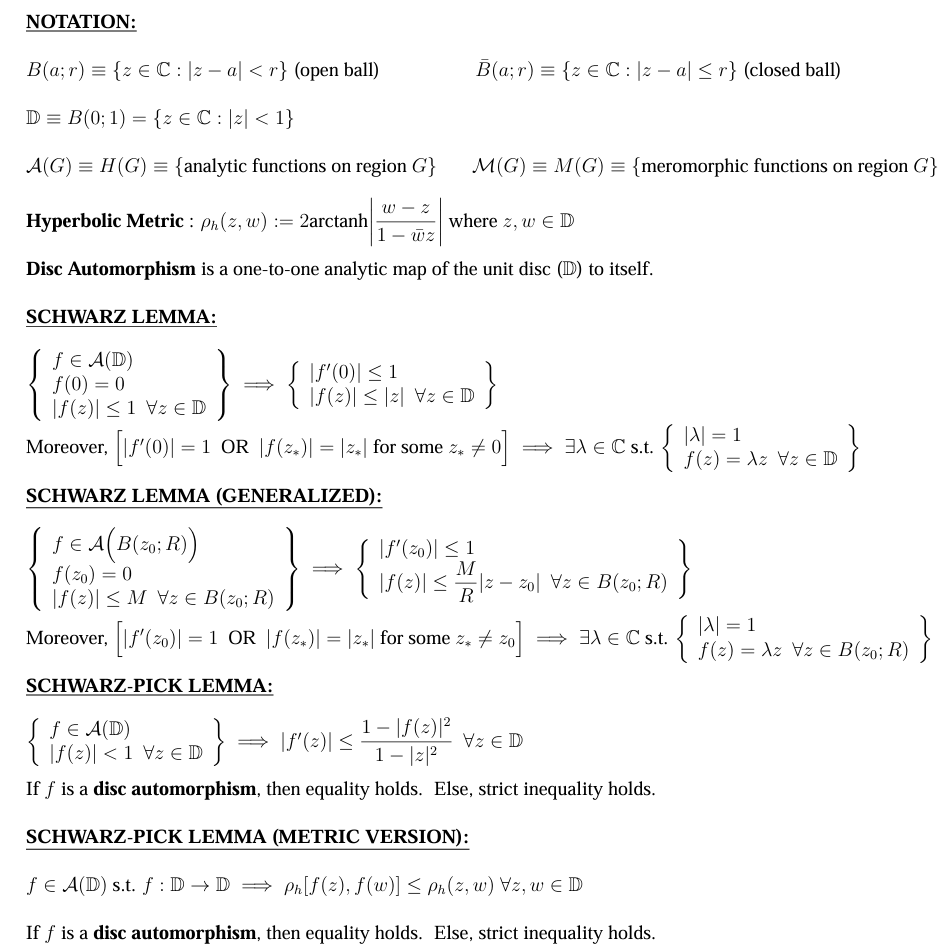
\includegraphics[width=\textwidth]{洛朗级数-2025041019.png}
% \caption{}
\label{}
\end{figure}

\subsection{Applications of Schwarz lemma}

\begin{exercise}[Stanford Ph. D test]
(b) Suppose that $f$ is analytic with $|f(z)|<1$ in $|z|<1$ and that $f( \pm a)=0$ where $a$ is a complex number with $0<|a|<1$. Show that $|f(0)| \leq a^2$. What can you conclude if this holds with equality.
\end{exercise}
\begin{proof}
Define
\[
F(z)=f(z) \cdot \frac{1-\overline{a} z}{z-a} \cdot \frac{1+\overline{a} z}{z+a}
\]
then $F(z)$ is analytic in $\{|z|<1\}$. When $|z|=1$,
\[
\left|\frac{1-\overline{a} z}{z-a} \cdot \frac{1+\overline{a} z}{z+a}\right|=1
\]
\[
\varlimsup_{|z| \rightarrow 1}|F(z)| \leq 1,
\]
which implies that $|F(z)| \leq 1$ for $|z|<1$. Take $z=0$, we obtain
\[
|f(0)| \leq|a|^2
\]
When it holds with equality, we have $F(z) \equiv e^{i \theta}$, which is equivalent to
\[
f(z)=e^{i \theta} \frac{z-a}{1-\overline{a} z} \cdot \frac{z+a}{1+\overline{a} z}
\]
\end{proof}

\begin{exercise}[Stanford]
(c) Determine all entire function $f$ that $\left|f^{\prime}(z)\right|<|f(z)|$.
\end{exercise}
\begin{proof}
(c) From $\left|f^{\prime}(z)\right|<|f(z)|$, we know that $f$ has no zero in $\mathbb{C}$, which implies that $\frac{f^{\prime}(z)}{f(z)}$ is also an entire function. It follows from $\left|\frac{f^{\prime}(z)}{f(z)}\right|<1$ that $\frac{f^{\prime}(z)}{f(z)}=c$, $|c|<1$. Integrating on both sides, we obtain $\log f(z)=c z+d$. Hence $f(z)=$ $c^{\prime} e^{c z}$, where $c$ and $c^{\prime}$ are constants and $|c|<1$.
\end{proof}
